\documentclass[11pt]{article}
\usepackage[T1]{fontenc}
\usepackage[utf8]{inputenc}
\usepackage{pgfplots}
\usepgfplotslibrary{external}
\usepgfplotslibrary{colorbrewer}
\pgfplotsset{
    % initialize Dark2
    cycle list/Dark2,
    % combine it with 'mark list*':
    cycle multiindex* list={
        mark list*\nextlist
        Dark2\nextlist
    },
    every axis plot/.append style={line width=1pt},
}
\pgfplotsset{compat=newest}
\usetikzlibrary{shapes.geometric}

\begin{document}

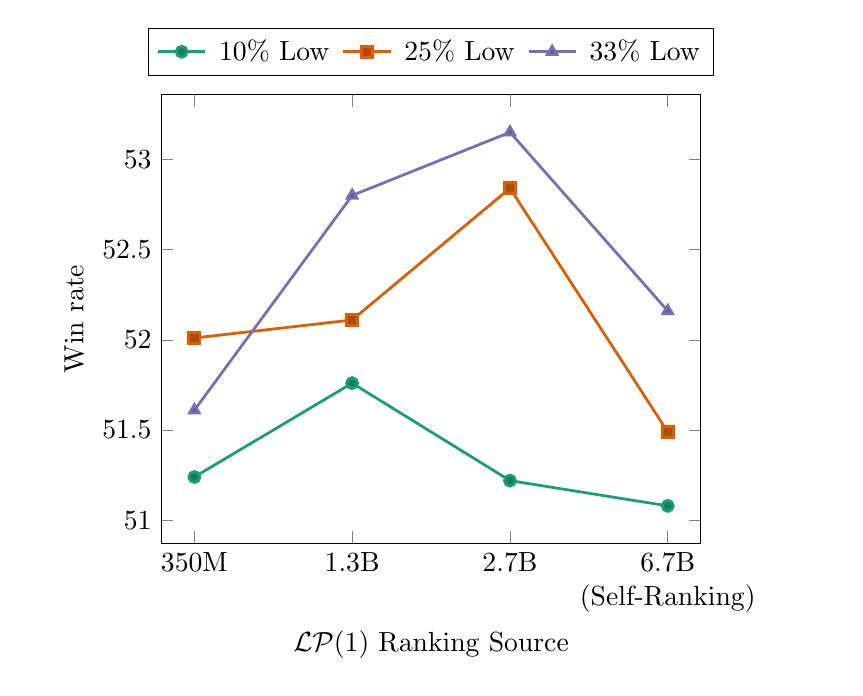
\begin{tikzpicture}
\begin{axis}[
    symbolic x coords={OPT 350M, OPT 1.3B,OPT 2.7B,OPT 6.7B},
    xticklabels={
        350M,
        1.3B,
        2.7B,
        6.7B\\(Self-Ranking)
    },
    xtick=data,
    xlabel=$\mathcal{LP}(1)$ Ranking Source,
    x tick label style={text width=4cm,align=center},
    legend style={at={(0.5,1.15)}, anchor=north, legend columns=3, legend cell align={left}, column sep=0.25em},
    ylabel=Win rate,
    enlarge y limits=0.1,
    enlarge x limits=0.07,
]
\addplot coordinates {
    (OPT 350M,51.24)
    (OPT 1.3B,51.76)
    (OPT 2.7B,51.22)
    (OPT 6.7B,51.08)
};
\addplot coordinates {
    (OPT 350M,52.01)
    (OPT 1.3B,52.11)
    (OPT 2.7B,52.84)
    (OPT 6.7B,51.49)
};
\addplot coordinates {
    (OPT 350M,51.61)
    (OPT 1.3B,52.80)
    (OPT 2.7B,53.15)
    (OPT 6.7B,52.16)
};
\legend{10\% Low, 25\% Low, 33\% Low}
\end{axis}
\end{tikzpicture}

\end{document}